\startchapter{Implementation}
\label{chapter:Exp}

%-- {\label{sec:method}}

\section{Building a Corpus}

To be effective, any approach that implements the Bertillonage philosophy
requires a corpus that is as comprehensive as possible. For Java, the
Maven2 Central Repository\footnote{http://repo1.maven.org/maven2/} fulfills
this requirement.  Maven2 provides a large public repository of reusable
Java components and libraries under various open source licenses, often
including multiple versions of each component; it serves as the Java
development community's de facto library archive.  Originally, the
repository was developed as a place from where the Maven build system could
download required libraries to build and compile an application.   Because
of the repository's broad coverage and depth, even competing dependency
resolvers make use of it (i.e., http://ant.apache.org/ivy/).
%as well as at least one commercial MSR
%tool\footnote{http://mvnrepository.com/}.

Maven2, as a whole, is unversioned: today's Maven2 collection will be
different from tomorrow's, as there is a continual accumulation of
artifacts.  Our first download of the Maven2 collection took place in June
of 2010 and our second download took place in July of 2011, over one year
later.  The repository grew substantially over this period, nearly doubling
in size.  This behaviour is unlike the major GNU/Linux compilations of free
and open source software such as Debian, where Debian 6.0 is a fixed
collection that remains essentially static
after its official release date.\footnote{
Debian does push critical security updates out to its stable releases,
but these usually represent the smallest possible changes necessary to patch
the discovered security holes.}


%wants to become a central
%repository that can be used for the dependency management tool Apache
%Maven\footnote{\url{maven.apache.org}}. There is little organization
%and no apparent documentation in terms of what goes into each of these
%directories.  For example, the directory \mytt{myfaces} contains two
%different copies of the same archive: \mytt{myfaces-1.0.9.jar} (one in
%the main directory and another one in the directory
%\mytt{myfaces-1.0.9}; on contrast version 1.0.10 is only present in
%the directory \mytt{myfaces-1.0.10}. It appears that, at this point,
%Maven2 is an stage of gathering Java code, before it is properly
%organized.



\section{Extracting the Class Signatures}
\label{subsec:extractSignature}

We developed two tools to extract anchored class signatures from Java
archives: a wrapper around \mytt{javac} for analyzing source code (using Oracle's 1.6.0\_20 version of \mytt{javac}),
and a byte code analyzer based on the \mytt{asm-3.3.1.jar} library.  Using these
tools we were able to consistently process interfaces, classes, methods,
fields, inner classes, enums, and generics.\footnote{We were unable to
process \emph{beta} implementations of generics sometimes found in Java 1.4
class files of a few brave bleeding edge developers from that time.}

When analyzing a source file we first call the \mytt{parse()} method of
\mytt{com.sun. tools.javac.main.JavaCompiler} that is contained inside
Java's \mytt{tools.jar}.  This parses the symbols of the source code
using the same logic as the command-line \mytt{javac} tool, but it stops
before resolving dependencies and compiling bytecode.  Once this is done,
we can recursively visit the class's symbols to extract fields, methods,
and inner classes.  We also perform several canonicalizations to ensure
signatures are extracted consistently, including:\footnote{Our source code
contains the full list of signature canonicalizations that we apply.
The source code is available to download from our replication package:

\url{http://juliusdavies.ca/2013/j.emse/bertillonage/}}


\begin{figure}
  \centering
  \begin{minipage}[h]{0.88\linewidth}
\hrule
\lstset{language=Java,
  tabsize=2,frame=none,
  keywordstyle=\color{darkblue},commentstyle=\color{darkgreen},stringstyle=\color{darkgreen},
  numbers=left,numberstyle=\scriptsize,numbersep=5pt,
  breaklines=true,showstringspaces=false,basicstyle=\scriptsize\ttfamily,emph={label}
}
\begin{lstlisting}
/*
 This small source file, A.java, is a valid Java program that
 generates 3 bertillonage signatures and 7 class files.

 We use this program to illustrate an asymmetry of Oracle's Java
 implementation: a single Java source file compiles into many
 binary class files should it contain inner-classes or sibling
 classes.
*/
public class A {
  Runnable r;

  public A() {
    // Anonymous inner-classes also compile into class files,
    // but our signature-extractor needs to ignore them.
    r = new Runnable() { public void run() {} };
  }

  // inner-classes A1, A2, A3.
  class A1 {}
  class A2 {}
  class A3 {}

}

// Sibling classes B and C. Notice they are outside class A.
class B {}
class C {}
\end{lstlisting}
\hrule\vspace{1mm}
\end{minipage}
  \caption{\small{Mapping source files to binary files is not always
straight-forward in Java.  This source file, \mytt{A.java},
despite its simplicity and small size, results in the
creation of 7 distinct class files due to
the inner-classes $A1, A2, A3$ and the anonymous class on line 16,
as well as the sibling-classes $B$ and $C$.
%Table~\ref{tab:asym} shows the results of compiling and analyzing
%this source file with our signature-extraction tool.
\vspace{-1em}}}
\label{lst:asym}
\end{figure}

\vspace{-0.5em}

\begin{itemize}

\item \emph{Remove explicit sub-classing of \mytt{java.lang.Object}}.
    Sometimes developers explicitly declare that a particular class ``extends Object''
    and \mytt{javac} faithfully reports back this fact.
    But all Java classes implicitly extend \mytt{java.lang.Object} according to
    the Java specification, so there is no point including this redundant
    information.

\vspace{0.3em}
\item \emph{Always mark interface methods as \mytt{public}}.
    Developers are free to leave off the \mytt{public} keyword on
    interface methods as a convenience, since all interface methods are
    public according to the Java specification.  However, we re-introduce
    the \mytt{public} keyword if it is missing to make the signature
    consistent with what is in the bytecode.

\vspace{0.3em}
\item \emph{Consistently deal with the \mytt{strictfp} keyword}.
    If the class is marked as \mytt{strictfp} then all its methods will
    be marked as \mytt{strictfp} in its bytecode, even if this modifier
    is missing in the source code for those same methods.

\end{itemize}


The approach we apply to bytecode is similar:  we call the \mytt{asm.jar}
bytecode analyzer to visit all fields, methods, and inner classes, and we
perform various canonicalizations to keep the bytecode signatures
consistent with source signatures.  When this process completes for both of
our two examples, \mytt{D.java}, and \mytt{D.class}, we should possess a
class signature identical to Figure~\ref{lst:cSig}.

Through the course of writing these tools we noticed a challenging
asymmetry of Java's implementation.  A source file will always contain
\emph{at least} one class, but it may contain several.  A class file,
however, contains the bytecode for \emph{at most} one complete class.
Class files never
include their own inner classes, which are stored as separate files.
For our tools this meant our source analyzer, when analyzing a
single file, might output many top-level class signatures.  On the other
hand, our binary analyzer, when pointed at a single file, often needed to
scan the archive or directory in question for additional files before it
could build a single signature.

\addtocounter{footnote}{1}

\footnotetext{These signatures are copied verbatim from the output of our extraction tool
after analyzing the \mytt{A.java} example (Figure~\ref{lst:asym}), and the class files were generated by running Oracle Java 1.6.0\_20's
\mytt{javac} against the same \mytt{A.java} file.}

\addtocounter{footnote}{-1}

\begin{table}[htbp]
  \centering
  \begin{tabular}{l|rl|r}
\textbf{One Source File} & \multicolumn{2}{l}{\textbf{Three Signatures\footnotemark}} & \textbf{Seven Class Files} \\
\hline
A.java & 1.  & \mytt{public class A}                               & A.class           \\
       &     & \mytt{~~Runnable r;}                                &                   \\
       &     & \mytt{~~public <init>()}                            &                   \\
       &     & \mytt{~~class A1}                                   & A\$A1.class       \\
       &     & \mytt{~~~~public <init>()}                          &                   \\
       &     & \mytt{~~class A2}                                   & A\$A2.class       \\
       &     & \mytt{~~~~public <init>()}                          &                   \\
       &     & \mytt{~~class A3}                                   & A\$A3.class       \\
       &     & \mytt{~~~~public <init>()}                          &                   \\
& & & \\
       & \multicolumn{2}{c|}{\emph{ignored anonymous inner-class}} & \emph{A\$1.class} \\
& & & \\
       & 2.  & \mytt{class B}                                      & B.class           \\
       &     & \mytt{~~<init>()}                                   &                   \\
& & & \\
       & 3.  & \mytt{class C}                                      & C.class           \\
       &     & \mytt{~~<init>()}                                   &                   \\
& & & \\
\hline
  \end{tabular}
  \vspace{1mm}
  \caption{This table shows how the small source file shown in Figure~\ref{lst:asym}
generates 3 anchored signatures when analyzed by our tool, and 7 class files when compiled.
In Java any given source file contains \emph{at least} one complete
class definition, whereas a binary file contains \emph{at most} one complete class
definition.  This asymmetry significantly complicated our own signature-extraction
tool's implementation.}
  \label{tab:asym}
\end{table}

Consider the code example in Figure~\ref{lst:asym}, \mytt{A.java}.
This small Java program contains only 11 source lines of code (SLOC) \cite{wheelerSloc},
and yet it compiles into 7 separate class files, and with our method it
contains 3 anchored signatures, as shown in Table~\ref{tab:asym}.
Even our baseline technique, where we calculate simple binary SHA1 fingerprints for each class,
is affected by this asymmetry:  we first must concatenate the outer class and all its inner
classes before running the SHA1 algorithm against the resulting binary data.



\vspace{-1em}
\section{Matching a Subject Artifact to Candidates} % Within the Corpus}

The source and bytecode tools we developed to extract the signatures are
employed both in the construction of a corpus index, as well as the
generation of queries to find matching candidates.  The two phases are
described below.

\textbf{Building the Corpus Index:}
we scan every source and binary archive within the Maven2 repository,
including archives within archives.  For each source and compiled class
file we compute its signature using the steps described in
section~\ref{subsec:extractSignature}.  To improve response time for
finding matches, we index each signature using its SHA1 hash.

\textbf{Finding Matches:}
we are interested in finding what archives have matching classes with the
subject, and what these classes are. To perform this step efficiently we
use the following algorithm:

\begin{compactenum}

\item For each class present in the subject, find its matching classes
    (with identical class signature) in the corpus.

\item Group the union of all matching classes (for all the classes in the
    subject) by their corresponding archive. This will result in a list of
    all archives that have at least one matching class with the subject,
    and for each archive, the list of matching classes with the subject.

\end{compactenum}

At this point we can now compute the similarity, inclusion, and containment
metrics of
the subject archive, compared with each of the archives that have at least one
matching class.  Table~\ref{tab:metricsExample} shows an example where a
subject artifact (\mytt{asm-2.2.3.jar}) is matched to candidate artifacts
within the corpus.

Note that even in an exact match the archive signature similarity index
might not be equal to $1$. This is because the source package might contain
some source Java files that are not included in the binary jar, such as
unit tests.  However, every class in the binary archive should be present
in the source archive, unless bytecode manipulators, or other post-compilation
processes alter the binary.

Nonetheless, even automatic code generation is likely to generate a well-defined set of
classes every time.
Our Bertillionage system already considers any output from these generators
to be ``copies" of each other. An improved Bertillionage system would
have to flag the common classes created by a generator as special, and
every time such copy is found, immediately mark its origin as known,
without having to check every other jar for matches. In fact, we see
this as the next step in Software Bertillionage: to create a curated
corpus of artifacts whose provenance is well known. Any candidate will
first be run against this corpus, and only if not match is found, run
against a the universal corpus (such as the one described in this
paper).


\section{Evaluating the Extractor and Exploring Maven2}
\label{sec:mavenExplore}

Initially we iteratively coded, tested and improved our extractor by
applying it against complete binary and source archives from a handful of
notable Java projects.  These included OpenOffice, Glassfish, Xerces, Xalan, Tomcat,
Eclipse, JBoss, the Rhino JavaScript engine, among others.
From across these diverse projects we identified 50 particularly
challenging source and binary pairs against which our tool, at various points,
failed to match the source and binary signatures.
All of these test files can be found in the \mytt{test-pairs} directory
of our tool.

These 50 pairs
became essentially our unit tests, and at this time only 2 of these
pairs fail to match, both from Xalan.
Releases of \mytt{xalan.jar} continue to be compiled
using a rare and hard-to-find IBM 1.3.1 Java compiler that is over 10 years old.
This compiler exhibits some strange behaviour with abstract classes
that happen to implement additional interfaces:
the compiler overriddes interface methods by ``pulling'' them down into the abstract class.
Since our tool is compiler-agnostic, there is no way for us to compensate for this signature-modifying behaviour.
The other failure comes from a Xalan auto-generated Java class that is
literally
named \mytt{CUP\$XPathParser\$actions}.  Our tool assumes the \mytt{\$} (dollar-sign) character is reserved for file names
of inner-classes.  Our assumption failed in this aforementioned case, but fixing this
problem would require significant effort on our part, as the assumption represents a core design decision within our tool.
We believe similar usage of \mytt{\$} in class names to be extremely rare in general,
as Oracle/Sun actively discourages such use in the Java Language Specification.

\begin{quote}
\emph{The \$ character should be used only in mechanically
generated source code or, rarely, to access preexisting names on legacy systems. \cite{jls2}}
\end{quote}


We decided to further evaluate the extractors that we had built as a kind of
validity check of our tools, as well as to explore the nature of what is
actually stored in the Maven2 repository.  To do so, we needed a set of
binaries for which we had ``ground truth''.  Consequently, we limited
ourselves to those binaries in the repository that had a corresponding
source code file in the same directory; that is, if the name of the binary
archive was \emph{name.jar}, then we required there to be a file named
\emph{name-sources.extension} in the same directory, where extension is one
of \emph{.zip}, \emph{.tar}, \emph{.war,} or \emph{.tgz}.

We picked a random sampling of 1,000 such Java binaries archives from
Maven2. Given the size of Maven2 --- there were 144,049 unique binary
packages at the time the work was done --- the size of this sample would
give us a  margin of error of 4\% with a confidence level of 99\%.  Each
binary archive was comprised of one or more Java classes; within our sample
set, we found that the median number of classes per binary archive was 10,
with an observed minimum of 1 class and an observed maximum of 2438
classes.

Naively, we expected that we should be able to find all of the binaries
with a perfect Similarity Index, and that we should also be able to find
the source of each.  We now discuss the results of our evaluation.

%-- \begin{itemize}
%-- \item Sampling of 1000 binary files from the repository.
%-- \item Each of them has a corresponding -source file in the same
%--   directory.
%-- \item We expect to match the binary with perfect Jaccard
%-- \item And also find the source
%-- \end{itemize}
%--
%-- Characteristics of the sample:
%--
%-- \begin{itemize}
%-- \item 1000 binary files.
%-- \item Min of 1 classes, maximum of 2438 classes, median of 10 classes.
%-- \end{itemize}

\subsection{Binary-to-binary matching results}
%-- Results: binary to binary

For each of the 1,000 archives in the sample set --- which of course we
knew to exist within the repository --- we computed its similarity with
every other binary archive in the repository.  Happily and unsurprisingly,
we found that in every instance they did indeed match themselves with a
Similarity Index value of 1.

To investigate the amount of duplication within Maven, we then asked:  For
each archive in the sample set, how many binary archives in Maven
repository matched it with a Similarity index of 1?  We found that the
median number of exact matches in our sample using the Similarity Index
measure was 5; that is, the binary occurred five times within the
repository, either on its own or contained within another archive.
However, we also found that many archives occurred a lot more often; the
maximum number within our sample set was 487 for
\mytt{servlet-api-2.5-6.1.12.jar}\footnote{Probably a file named
\mytt{servlet-api-2.5.jar} is the true origin of this large equivalence
class of perfect matches.  JSP \& Servlet technologies have long been
an important part of Java's popularity in servers for over 10 years,
and \mytt{servlet-api-2.5.jar} is a critical interface library
which all Java web and application servers must implement, including Tomcat, JBoss,
Glassfish, Jetty, and many others.  The 6.1.12 in this case probably
comes from a version of Jetty.  The Jetty project tends to rename its own critical
dependencies so that they contain Jetty's own version number alongside
the original dependency's version number.}

We also considered the inclusion and containment measures for our sample
set.  Inclusion and containment occur when one archive is a superset of another; this is
often the result of an archive owner deciding to include dependent archives
within it, to ease subsequent deployment.
By our definition, inclusion and containment are inverses of each other:
\emph{inclusion($A,B$)} $=$ \emph{containedBy($B,A$)}.

Figure~\ref{fig:topMatchesSource} summarizes the results of all three
measures on our sample set.  For most jars, the number of matches was small
(median 5), but a few jars had very large number of matches. This was
usually because there were either many copies of the archive, or
the signature of the archive matched several versions (i.e., the original
source code had not changed signature in several versions).

When the top Inclusion index contains many matches this suggests that this
is a ``super-jar'' that contains classes found in other archives, not only
the one sought (they include their dependencies in the same jar).  When the
top Containment index returns many matches, this suggest that the classes
in a binary archive that tends be embedded in many other jars.

As we expected, Inclusion and Containment had longer tails than the
Similarity Index.  In our sample set, the archive with the largest number
of inclusions was \mytt{easybeans-example-pool-1.1.0-M1b-JONAS.jar} with
864 matches (i.e., it contains 864 other archives), and the archive that
was contained most often by other archives was
\mytt{maven-classpath-plugin-1.2.6-jar-with-dependencies.jar} with 2732
inclusions (i.e., it is fully contained within 2732 other archives).  Maven
reliability and duplication is discussed in Section
\ref{sec:mavenreliability}.

%-- \begin{itemize}
%-- \item Ideally, we should be able to match each to their corresponding
%--   binary with Jaccard == 1, indeed, all they do.
%-- \item How many packages match the same signature? This will give us a
%--   metric of duplication in maven. See figure \ref{fig:matchesMetric}.
%--
%-- How to read this:
%--     \begin{itemize}
%--     \item Most packages have few copies (Jaccard median of 5) but many of
%-- 	them have a lot. For example, the maximum, with 487 copies is
%-- 	servlet-api-2.5-6.1.12.jar.
%--
%--     \item As expected, Inclusion and Containment have longer tails: For
%-- 	example, the largest inclusion is
%-- 	easybeans-example-pool-1.1.0-M1b-JONAS.jar, with 864 matches (it
%-- 	contains 864 other packages) and for containment it is
%-- 	maven-classpath-plugin-1.2.6-jar-with-dependencies.jar with 2732
%-- 	(it is fully contained in 2732 other packages). In other words
%--
%--     \item Inclusion tell us when a package is a superset of another. This
%-- 	is probably a result of including the dependencies of the package
%-- 	in it.
%--
%--     \item Containment tell us when a package is a subset of another. This
%-- 	is probably the result of a package being incorporated (as a
%-- 	dependency) in another.
%--
%--     \end{itemize}
%-- \end{itemize}

\begin{figure}[h]
  \centering
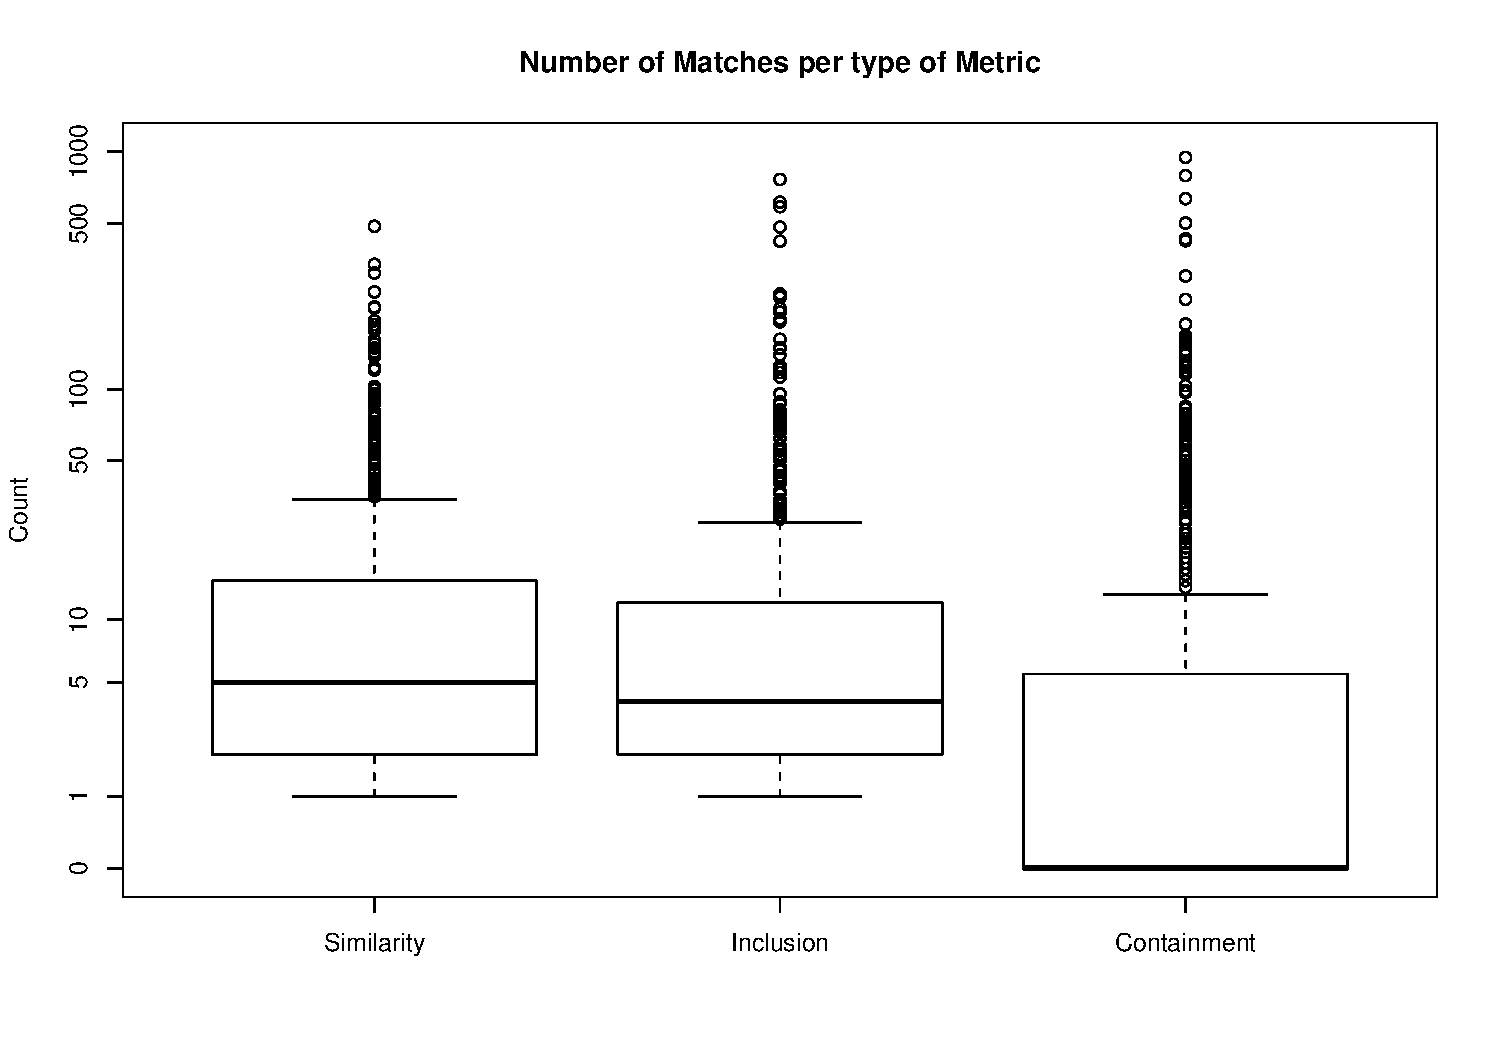
\includegraphics[width=\columnwidth]{plots/boxplotPerfectMatches.pdf}
\vspace{-7mm}
  \caption{Number of top-matches found in the binary-to-binary
    experiment. The different metrics had a median of 5 or 6 matches,
    but they had long tails, suggesting a lot of duplication of some
    jars in the sample. }
  \label{fig:topMatchesSource}
\end{figure}


\subsection{Binary-to-source matching results}
%-- Results, binary to source.

For each of the 1,000 archives in the sample set we computed its similarity
with every source archive in the repository.  While we satisfied ourselves
that our extractors worked as expected, the exploration of the Maven
repository yielded some surprising results:

We classify the result of a search into three three categories:

    \begin{enumerate}
    \item The correct match was among those with the top matching Similarity
	index (966 cases out of 1,000).
    \item The correct match had a lower Similarity index than some
	other archives (30 cases).
    \item The algorithm failed to suggest any matches (4 cases).
    \end{enumerate}

In 966 of the 1,000 archives in the sample set, the correct match was among
those with the top Similarity Index.  The median Similarity Index of a
binary archive and its corresponding source archive was 1.0.  However,
there were several cases where the correct source match had a surprisingly
low Similarity Index, with the lowest in our sample set being 0.0290.  Low
Similarity indexes typically indicate that dependent archives have been
added within the binary version of the archive; for example, the source
Java files in \mytt{rampart-integration-1.5.1.jar} have 12 signatures, yet
its binary version contains 231 signatures (those of classes it uses as
dependencies, and that are embedded in the jar to avoid having to
independently install them in the running environment).  The distribution
of the top number of source packages matching the top Inclusion Index is
shown in figure~\ref{fig:topMatchesSource}.

If there are multiple top matches for a given archive --- that is, if there
are multiple archives with the same maximal Inclusion index when compared
to the candidate archive --- then a more detailed examination of them must
be performed.  Typically, this means that there are multiple versions of
the archive that have an identical interface; that is, the implementation
may have evolved between versions but the interface stayed consistent.  In
our sample set, we found that the minimum number of top matches was 1, and
the median was 4.  However, there were a few cases where the number of top
matches was large; the most extreme case was
\mytt{maven-interceptor-1.380.jar} for which we found 158 different
versions from 1.237 to 2.0.1.

We were not able to match any source in 4 cases.  These were all small
archives consisting of between one and three classes each, and in each of
these cases the compiler, or other bytecode manipulators had added various
fields and methods that were not actually in the source code.  While we are
aware of this phenomenon, our extractor does not explicitly handle such
fields and methods.


And finally, we noted that in 30 cases, the top match was not the correct
match.  Manual inspection suggests that in these cases the binary jars had
embedded within them external dependencies from other archives whose
numbers exceeded those of the source itself.  For example,
\mytt{org.apache.felix. http.bundle-2.0.2-sources.jar} contains only one
Java file, yet its binary equivalent \mytt{org.apache.felix.http.bundle.2.0.2.jar}
contains 295 signatures (in 442 .class files); other binary
packages with a higher Inclusion Index were \mytt{servlet-api-2.5}
(contributing 145 signatures) and \mytt{jetty-6.1.*}, contributing 13
classes.  This brings up an interesting philosophical question: What is the
source of a given binary?  Is it the source it was created from, or the
dependencies it contains?  Certainly all of them, and our method shows
this.

Of these 30 cases, 10 source files have a Containment Index of 1.0 (their
binary jar perfectly contains all the signatures in the source file). In
other words, while the expected source was not the top match for the
Similarity Index, it was for the Containment one.

%  \migod{Below are Daniel's original comments, which I need some help
% understanding.}

% Not top match: 30. In other words, for 30 jars the source file
%   in the same directory was not the best match. We analyze few of
%   these files, and discovered that the main reason they did not match is
%   because the binary jars are also embedding dependencies from other
%   packages, and these dependencies are larger than the source itself. For
%   example, \mytt{org.apache.felix.http.bundle-2.0.2-sources.jar} contains
%   only 1 Java file, yet its binary equivalent:
%   \mytt{org.apache.felix.http.bundle-2.0.2.jar} contains 295 signatures (in
%   442 .class files). The Bertillonage metrics show that it contains 41
%   files from \mytt{servlet-api-2.5}, and 145 and from jetty-6.1.*., 13
%   classes from \mytt{org.apache.felix.http.whiteboard-2.0.*}.

%   This really brings something interesting: what is the source of the
%   binary? Is it the one that created it, or the dependencies it contains?
%   Certainly both, and the Bertillonage metrics show it.

%   Of there 30 cases, 10 source files have a Containment metric of 1.0
%   (they binary jar perfectly contains all the signatures in the source
%   file).

%-- \begin{itemize}
%-- \item Top match: 966. For these, the expected source was listed as the top
%--     match. The values are: Min.  :0.0290 , Median 1.00, Max, 1.000. In
%--     fact, only 10\% (98) had a Jaccard less than 1. Those with low Jaccard
%--     reflected packages that included dependencies into the binary (e.g.
%--     \mytt{rampart-integration-1.5.1.jar} has 12 signatures, yet it binary
%--     has 231 ones). The distribution of the top number of source packages
%--     matching the top Jaccard is shown in figure~\ref{fig:topMatchesSource}.
%--     At is can be seen, the median number of top matches is very small:
%--     min1, max 158, median 4, but in few cases.  The largest set of matches
%--     (158) correspond to \mytt{maven-interceptor-1.380.jar} to 158 different
%--     versions of it, from 1.237 to 2.0.1.
%--
%-- \item We were not able to match any source in 4 cases. The reasons are:
%--     very small packages (1,1,2, and 3 classes) for which the compiler adds
%--     fields and methods to the class that are not in the source. These are
%--     not handled by our parser.

%/maven/org/ow2/jasmine/monitoring/jasmine-monitoring-integration-tests-modules-events/1.2.5/jasmine-monitoring-integration-tests-modules-events-1.2.5.jar
%/maven/org/ow2/jasmine/monitoring/jasmine-monitoring-integration-tests-modules-events/1.2.5/jasmine-monitoring-integration-tests-modules-events-1.2.5-sources.jar
%
%This one has some fields in the class that are not in the source:
%
%f;0;  private InstanceManager __IM;
%f;0;  private boolean __Flogger;
%...
%f;0;  private boolean __Mstart;
%m;0;  Logger __getlogger()
%m;0;  void __setlogger(Logger)
%-- \item Not top match: 30. In other words, for 30 jars the source file
%--   in the same directory was not the best match. We analyze few of
%--   these files, and discovered that the main reason they did not match is
%--   because the binary jars are also embedding dependencies from other
%--   packages, and these dependencies are larger than the source itself. For
%--   example, \mytt{org.apache.felix.http.bundle-2.0.2-sources.jar} contains
%--   only 1 java file, yet its binary equivalent:
%--   \mytt{org.apache.felix.http.bundle-2.0.2.jar} contains 295 signatures (in
%--   442 .class files). The Bertillonage metrics show that it contains 41
%--   files from \mytt{servlet-api-2.5},  and 145 and from jetty-6.1.*., 13
%--   classes from \mytt{org.apache.felix.http.whiteboard-2.0.*}.
%--
%--   This really brings something interesting: what is the source of the
%--   binary? Is it the one that created it, or the dependencies it contains?
%--   Certainly both, and the Bertillonage metrics show it.
%--
%--   Of there 30 cases, 10 source files have a Containment metric of 1.0
%--   (they binary jar perfectly contains all the signatures in the source
%--   file).
%--
%-- \end{itemize}


\begin{figure}[h]
  \centering
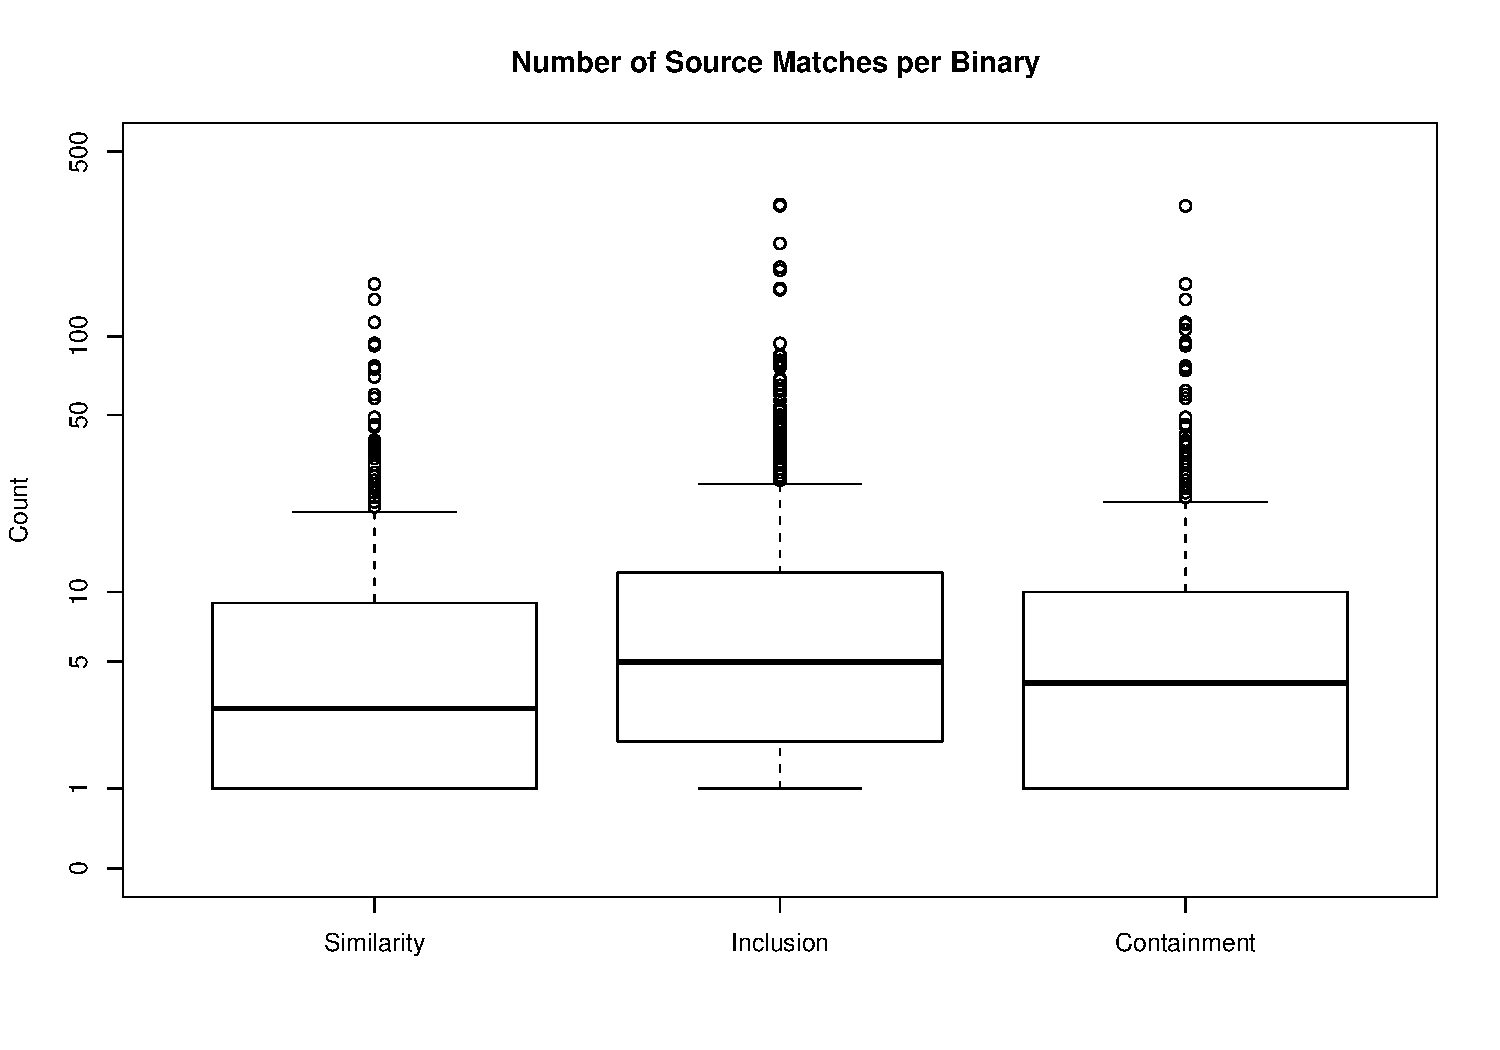
\includegraphics[width=\columnwidth]{plots/boxplotAllMatches.pdf}
\vspace{-7mm}
  \caption{Matching sources: Number of matches for each metric}
  \label{fig:matchesMetric}
\end{figure}


\subsection{Summary of Exploration and Tool Evaluation}

In summary, to evaluate our tools and to explore the problem space
of the Maven repository, we applied our techniques to 1,000 binary
archives, randomly chosen from Maven but with the constraint that the
sources also be present in Maven.  In 96.6\% of the cases (margin of
error of 4\% with a confidence level of 99\%) we were able to match
the binary of a source using (one of) the top Similarity Index
match(es). In 3\% of the cases the best match was not the correct
source (but the correct one had a slightly lower similarity index and
was part of the set of candidates). In 0.4\% of the cases, we could not match
the source at all.
% ; however, in
% each of these cases the archives were very small so manual matching
% would be quick.

Overall, our metrics-based approach appears to be effective for
significantly narrowing the search space when looking for matches for
another binary (the median number of top matches was 5). In the few
occasions it failed to find a match (0.4\%), the archives were very small
and the compiled classes were built using features (e.g., direct bytecode
manipulation) that our parser was not able to process.

When matching binary packages to their corresponding source, we identified
several commonalities. In many cases, the binary and the source were a
1-to-1 match, but in many other cases, the binary was a superset of the
source archive (it contained the dependencies that it required to
function). In this case, the containment metric is useful: it shows us that
the binary package contains the source packages.  We found it interesting
that in few cases, the best-match was not the corresponding source, but one
of its dependencies.  In other cases, the best match was a subset of the
binary archive. This is common when a source archive is split into several
binary packages, or when there exists a large number of test cases that are
not included in the binary. In these cases the inclusion metric is the best
to use.

% \begin{itemize}
% \item Overall, the Jaccard metric is a very effective method to narrow
%   the search space when looking for the source code of a binary. The
%   median number matches one would need to analyze was 5.
% \item In many cases a binary package would contain classes not present
%   in the sources. These are typically dependencies. Sometimes these
%   dependencies might be more numerous than the number of Java files in
%   its source. The Jaccard and Inclusion metric can be very useful to
%   identify such packages.
% \item Some binary packages are ``super containers'' that are composed
%   of numerous binaries that come from different products.
% \item For very few packages, the signatures do not change over a long
%   period of time.
% \end{itemize}

